% ============================================================================
% ASTROMANAGER v1.3.0 — USER MANUAL (English)
% ============================================================================
% Compile with:  pdflatex USER_MANUAL_EN.tex && pdflatex USER_MANUAL_EN.tex
% (two passes for table of contents)
% ============================================================================

\documentclass[11pt,a4paper]{article}

% ── Encoding & Language ──
\usepackage[utf8]{inputenc}
\usepackage[T1]{fontenc}
\usepackage[english]{babel}

% ── Page geometry ──
\usepackage[margin=2.5cm,headheight=14pt]{geometry}

% ── Fonts ──
\usepackage{lmodern}
\usepackage{microtype}

% ── Colors ──
\usepackage[table,dvipsnames]{xcolor}
\definecolor{mainblue}{HTML}{1a3a5c}
\definecolor{accentcyan}{HTML}{94b8c8}
\definecolor{warningorange}{HTML}{c0b098}
\definecolor{bgdark}{HTML}{0a0e1a}
\definecolor{successgreen}{HTML}{88b098}
\definecolor{errorcoral}{HTML}{b89090}
\definecolor{infogrey}{HTML}{90a8b8}
\definecolor{rowlight}{HTML}{EDF2F7}
\definecolor{rowdark}{HTML}{D9E2EC}
\definecolor{linkblue}{HTML}{2a6a9c}

% ── Tables ──
\usepackage{booktabs}
\usepackage{colortbl}
\usepackage{array}
\usepackage{longtable}
\usepackage{tabularx}

% ── Boxes ──
\usepackage[skins,breakable]{tcolorbox}
\tcbset{
    boxrule=0.5pt,
    arc=3pt,
    fonttitle=\bfseries,
    left=6pt,
    right=6pt,
    top=4pt,
    bottom=4pt,
}

% Tip box (blue)
\newtcolorbox{tipbox}[1][Tip]{
    colback=mainblue!8,
    colframe=mainblue!70,
    coltitle=white,
    colbacktitle=mainblue!80,
    title={#1},
    fonttitle=\bfseries\small,
}

% Warning box (orange)
\newtcolorbox{warningbox}[1][Warning]{
    colback=warningorange!15,
    colframe=warningorange!80!black,
    coltitle=white,
    colbacktitle=warningorange!80!black,
    title={#1},
    fonttitle=\bfseries\small,
}

% Note box (grey-blue)
\newtcolorbox{notebox}[1][Note]{
    colback=accentcyan!10,
    colframe=accentcyan!60,
    coltitle=white,
    colbacktitle=accentcyan!70!black,
    title={#1},
    fonttitle=\bfseries\small,
}

% Critical box (red)
\newtcolorbox{criticalbox}[1][Critical]{
    colback=errorcoral!10,
    colframe=errorcoral!70!black,
    coltitle=white,
    colbacktitle=errorcoral!70!black,
    title={#1},
    fonttitle=\bfseries\small,
}

% New-feature box (green)
\newtcolorbox{newfeaturebox}[1][New in v1.2.0]{
    colback=successgreen!10,
    colframe=successgreen!70!black,
    coltitle=white,
    colbacktitle=successgreen!60!black,
    title={#1},
    fonttitle=\bfseries\small,
}

% ── Headers & Footers ──
\usepackage{fancyhdr}
\pagestyle{fancy}
\fancyhf{}
\fancyhead[L]{\small\textcolor{mainblue}{\textbf{AstroManager v1.3.0} --- User Manual}}
\fancyhead[R]{\small\textcolor{mainblue}{\nouppercase{\leftmark}}}
\fancyfoot[C]{\small\textcolor{mainblue}{\thepage}}
\renewcommand{\headrulewidth}{0.4pt}
\renewcommand{\footrulewidth}{0pt}
\renewcommand{\headrule}{\hbox to\headwidth{\color{mainblue}\leaders\hrule height \headrulewidth\hfill}}

% ── Hyperlinks ──
\usepackage{hyperref}
\hypersetup{
    colorlinks=true,
    linkcolor=mainblue,
    urlcolor=linkblue,
    citecolor=mainblue,
    pdfauthor={AstroManager},
    pdftitle={AstroManager v1.3.0 -- User Manual},
    pdfsubject={Astrophotography File Management},
    pdfkeywords={FITS, XISF, astrophotography, PyQt6, quality analysis, WBPP},
    bookmarksnumbered=true,
}

% ── Graphics ──
\usepackage{graphicx}

% ── Lists ──
\usepackage{enumitem}
\setlist{nosep, leftmargin=1.5em}

% ── Section styling ──
\usepackage{titlesec}
\titleformat{\section}
    {\Large\bfseries\color{mainblue}}
    {\thesection}{0.8em}{}[\vspace{-0.3em}\textcolor{mainblue}{\rule{\textwidth}{0.5pt}}]
\titleformat{\subsection}
    {\large\bfseries\color{mainblue!80!black}}
    {\thesubsection}{0.6em}{}
\titleformat{\subsubsection}
    {\normalsize\bfseries\color{mainblue!60!black}}
    {\thesubsubsection}{0.5em}{}

% ── Misc ──
\usepackage{parskip}
\setlength{\parskip}{0.5em}
\setlength{\parindent}{0pt}

% ── Code / monospace ──
\usepackage{fancyvrb}
\DefineVerbatimEnvironment{codeblock}{Verbatim}{
    fontsize=\small,
    frame=single,
    rulecolor=\color{mainblue!30},
    xleftmargin=0.5em,
    xrightmargin=0.5em,
}

% ── Alternating row color helper ──
\newcommand{\rowmark}{\rowcolor{rowlight}}

% ============================================================================
% DOCUMENT
% ============================================================================

% ===================================================================
% Format maison des PDF (14/10/2026) : titres sans-serif colorés (sky,
% alert), en-tête et pied sobres, anti-titres orphelins, captures réelles.
% Les noms de couleurs historiques sont ramenés à la palette maison.
% ===================================================================
\usepackage{needspace}
\usepackage{listings}
\usepackage{tabularx}
\usepackage{booktabs}
\usepackage{etoolbox}
\usepackage{fontawesome5}
\input{version}
\definecolor{sky}{HTML}{1C6DB4}
\definecolor{skyl}{HTML}{E6F0F9}
\definecolor{alert}{HTML}{B5382B}
\definecolor{steppe}{HTML}{C08A2E}
\definecolor{summit}{HTML}{6B7A8F}
\definecolor{night}{HTML}{232A56}
\definecolor{forest}{HTML}{2E7D5B}
\definecolor{ink}{HTML}{1F2430}
\definecolor{mainblue}{HTML}{1C6DB4}
\definecolor{accentcyan}{HTML}{6B7A8F}
\definecolor{warnorange}{HTML}{C08A2E}
\definecolor{successgreen}{HTML}{2E7D5B}
\definecolor{errorcoral}{HTML}{B5382B}
\definecolor{infogrey}{HTML}{6B7A8F}
\definecolor{titlegold}{HTML}{C08A2E}
\definecolor{linkblue}{HTML}{1C6DB4}
\definecolor{tablegray}{HTML}{E6F0F9}
\definecolor{tablealt}{HTML}{F5F8FB}
\AtBeginDocument{\color{ink}}
\titleformat{\section}
  {\Large\bfseries\sffamily\color{sky}}
  {\thesection}{0.6em}{}
  [{\vspace{1pt}\color{sky!35}\titlerule[1.3pt]}]
\titlespacing*{\section}{0pt}{16pt}{8pt}
\titleformat{\subsection}{\large\bfseries\sffamily\color{alert}}{\thesubsection}{0.5em}{}
\titlespacing*{\subsection}{0pt}{12pt}{4pt}
\titleformat{\subsubsection}{\normalsize\bfseries\sffamily\color{night}}{\thesubsubsection}{0.5em}{}
\pretocmd{\section}{\needspace{12\baselineskip}}{}{}
\pretocmd{\subsection}{\needspace{6\baselineskip}}{}{}
\pretocmd{\subsubsection}{\needspace{5\baselineskip}}{}{}
\raggedbottom
\setlength{\emergencystretch}{3em}
\fancyhf{}
\renewcommand{\headrulewidth}{0.4pt}
\renewcommand{\footrulewidth}{0pt}
\renewcommand{\headrule}{\hbox to\headwidth{\color{sky!40}\leaders\hrule height \headrulewidth\hfill}}
\fancyhead[L]{\sffamily\small\color{sky}\textbf{AstroManager} \color{summit}\textbar{} User manual}
\fancyhead[R]{\sffamily\small\color{summit}\thepage}
\fancyfoot[C]{\sffamily\scriptsize\color{summit}Version \VERSIONAPP{} \textbar{} github.com/ARP273-ROSE/astromanager}
\graphicspath{{../captures/}{../../assets/}}
\newcommand{\capture}[2][0.92]{\par\needspace{16\baselineskip}\begin{center}\setlength{\fboxsep}{0pt}\setlength{\fboxrule}{0.6pt}%
  \fcolorbox{summit!50}{white}{\includegraphics[width=\dimexpr#1\linewidth-1.3pt\relax]{#2}}\end{center}}
\newcommand{\menu}[1]{\textsf{\textbf{\textcolor{sky}{#1}}}}

\begin{document}

% ============================================================================
% TITLE PAGE
% ============================================================================
\begin{titlepage}
\thispagestyle{empty}
\vspace*{1.4cm}
\begin{center}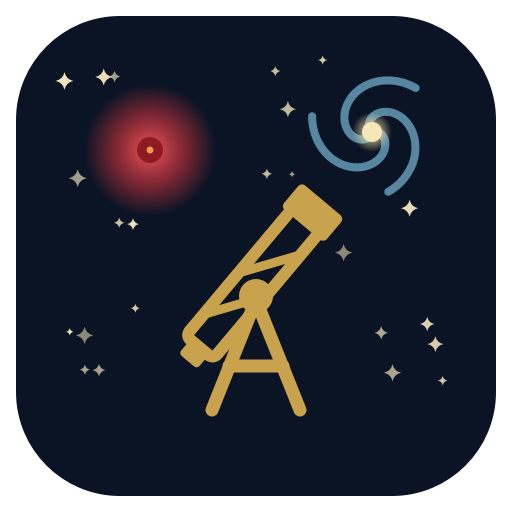
\includegraphics[width=4.6cm]{icon_512.png}\end{center}
\vspace{8mm}
{\sffamily\color{summit}\large AstroManager\par}
\vspace{4mm}
{\color{sky!35}\hrule height 2pt}
\vspace{7mm}
{\sffamily\bfseries\color{sky}\fontsize{26}{30}\selectfont User manual\par}
\vspace{4mm}
{\sffamily\color{night}\large Astrophotography file manager and analyser\par}
\vspace{7mm}
{\color{sky!35}\hrule height 2pt}
\vspace{5mm}
{\sffamily\color{summit}\normalsize Version \VERSIONAPP\par}
\vfill
{\sffamily\small\color{summit} MIT \textbar{} github.com/ARP273-ROSE/astromanager\par}
\end{titlepage}

% ============================================================================
% TABLE OF CONTENTS
% ============================================================================
\newpage
\pagenumbering{roman}
\tableofcontents
\newpage
\pagenumbering{arabic}

% ############################################################################
% SECTION 1 — INTRODUCTION
% ############################################################################
\section{Introduction}
\label{sec:introduction}

\subsection{What is AstroManager?}

AstroManager is a comprehensive, professional-grade file management suite designed specifically for astrophotographers. Built with Python and PyQt6, it provides a modern, cosmic-themed interface with \textbf{18 organized tabs} covering every aspect of astrophotography data management:

\begin{itemize}
    \item Universal file analysis (FITS, XISF, FITS.FZ)
    \item Multi-codec compression with 9 profiles
    \item Mass header editing with NINA compatibility
    \item Flat frame management and coverage tracking
    \item Frame quality analysis with PSF fitting and star detection
    \item WBPP-ready export with automatic calibration matching
    \item Target tracking over time with SIMBAD integration
    \item Interactive celestial sky chart
    \item Observation shoot calendar with heatmap
    \item PixInsight log analysis
    \item Mount tracking analysis (MountMonitor)
    \item Observation history and statistics dashboard
    \item Built-in database browser (cameras, telescopes, filters, targets)
    \item Disk space analysis and duplicate detection
    \item ASIAIR import workflow
    \item N.I.N.A. CSV analytics with correlation analysis and efficiency tracking
    \item FITS/XISF image viewer with FWHM heatmap, corner inspector, STF autostretch
    \item Cross-section comparison with filter attenuation analysis and auto-alignment
\end{itemize}

AstroManager handles \textbf{200,000+ files} efficiently through parallel processing, multi-tier caching, and automatic hardware detection.

\subsection{Supported Formats}

\begin{center}
\rowcolors{2}{rowlight}{white}
\begin{tabular}{llp{7cm}}
\toprule
\textbf{Format} & \textbf{Extension} & \textbf{Description} \\
\midrule
FITS & \texttt{.fits}, \texttt{.fit}, \texttt{.fts} & Standard astronomical image format \\
XISF & \texttt{.xisf} & PixInsight native format with XML metadata \\
FITS.FZ & \texttt{.fits.fz}, \texttt{.fz} & RICE tile-compressed FITS (fpack) \\
\bottomrule
\end{tabular}
\end{center}

\subsection{System Requirements}

\begin{center}
\rowcolors{2}{rowlight}{white}
\begin{tabular}{lp{10cm}}
\toprule
\textbf{Component} & \textbf{Requirement} \\
\midrule
Python & 3.8 or newer (3.11+ recommended) \\
Operating System & Windows 10/11, Linux (Ubuntu 20.04+, Manjaro, etc.), macOS 12+ \\
RAM & 4\,GB minimum, 8\,GB+ recommended for large datasets \\
Storage & SSD recommended for best performance \\
GUI Framework & PyQt6 6.2+ \\
Core Libraries & numpy, astropy, matplotlib, pandas, Pillow, reportlab, tqdm, requests, xisf \\
Optional & scipy (PSF fitting, DBSCAN), astroquery (SIMBAD), psutil (auto-tuning), zstandard, lz4, pyqtgraph$\geq$0.13 (GPU viewer), photutils$\geq$1.5 (DAOStarFinder), astroalign (auto-alignment), scikit-image (phase correlation) \\
\bottomrule
\end{tabular}
\end{center}

\subsection{What's New in v1.2.0}

Version 1.2.0 is a major feature release inspired by \href{https://github.com/eg013ra1n/rustafits}{Athenaeum/rustafits} (Vilen Sharifov). It introduces five new tabs and several cross-cutting features:

\begin{newfeaturebox}[New Tabs in v1.2.0]
\begin{itemize}
    \item \textbf{Quality Analysis} --- Per-frame star detection, 2D PSF Moffat/Gaussian fitting, quality scoring 0--100, satellite trail detection, interactive star maps
    \item \textbf{WBPP Export} --- PixInsight WBPP-ready folder organization with 8-parameter calibration matching, scoring 0--1, template tokens, and preview tree
    \item \textbf{Sky Chart} --- Aitoff/Mollweide projection of all targets, color-coded by object type, filter, or integration time, with Milky Way band overlay
    \item \textbf{Calendar} --- Monthly grid and yearly GitHub-style heatmap of imaging sessions with statistics dashboard
    \item \textbf{Tags \& Workflow} --- Colored tags and Stage/WIP/Archive workflow stages for target classification
\end{itemize}
\end{newfeaturebox}

\begin{newfeaturebox}[New Cross-Cutting Features in v1.2.0]
\begin{itemize}
    \item \textbf{DBSCAN Clustering} --- Automatic target deduplication by RA/Dec coordinates using DBSCAN with Haversine distance
    \item \textbf{Database Schema v4} --- New tables for tags, workflow stages, and frame quality cache
    \item \textbf{Batch Plate Solving} --- Solve all unsolved raw LIGHT frames in one click, with in-place XISF header update
\end{itemize}
\end{newfeaturebox}

\subsection{What's New in v1.3.0}

Version 1.3.0 adds three major analytical tabs, each inspired by a dedicated open-source astrophotography project. Together they bring imaging session analytics, deep image inspection, and comparative filter analysis into a single integrated suite.

\begin{newfeaturebox}[New Tabs in v1.3.0]
\begin{itemize}
    \item \textbf{Analytics} --- N.I.N.A. CSV import, imaging efficiency vs.\ astronomical dark time, metric correlations (HFR, FWHM, eccentricity vs.\ temperature, humidity, wind), time-series trending with moving averages, and per-equipment performance statistics. Inspired by \href{https://github.com/chvvkumar/GalactiLog}{GalactiLog} (chvvkumar).
    \item \textbf{Image Viewer} --- FITS/XISF browser with GPU-accelerated display (pyqtgraph), PixInsight-style STF autostretch, FWHM heatmap with Nadaraya--Watson kernel regression, 3$\times$3 corner inspector with per-cell quality grading, and star overlay. Inspired by \href{https://github.com/ricksastro/Astronalyze}{Astronalyze} (ricksastro).
    \item \textbf{Cross-Section} --- Side-by-side dual image viewer with line profile comparison, histogram overlay, filter attenuation analysis (Welch t-test, Cohen's d, SNR, exposure factor), and star-based auto-alignment via astroalign. Inspired by \href{https://github.com/brentmantooth/AstroCrossSections}{AstroCrossSections} (brentmantooth).
\end{itemize}
\end{newfeaturebox}

\begin{newfeaturebox}[New Cross-Cutting Features in v1.3.0]
\begin{itemize}
    \item \textbf{Database Schema v5} --- New tables for N.I.N.A. exposure data, weather correlation, imaging efficiency, session notes, and equipment performance tracking
    \item \textbf{Session Notes} --- Per-date text notes with target association, saved in the database for long-term annotation of imaging sessions
    \item \textbf{Target Resolver} --- Automatic SIMBAD coordinate lookup when importing N.I.N.A. CSV data
\end{itemize}
\end{newfeaturebox}


% ############################################################################
% SECTION 2 — INSTALLATION
% ############################################################################
\section{Installation}
\label{sec:install}

\subsection{The installer (recommended)}

Ready-to-use packages, Python and every dependency included, are published on
the releases page:
\url{https://github.com/ARP273-ROSE/astromanager/releases/latest}. No
administrator rights are needed: everything installs into your own profile.

\begin{center}
\begin{tabularx}{\linewidth}{@{}l>{\raggedright\arraybackslash}X@{}}
\toprule
\textbf{System} & \textbf{File and first launch} \\
\midrule
Windows & \texttt{AstroManager-Setup.exe}. If SmartScreen warns that the
installer is unsigned: \emph{More info}, then \emph{Run anyway} (only once). \\
macOS & \texttt{AstroManager-X.Y.Z-macos-arm64.dmg} (Apple Silicon) or
\texttt{-macos-x86\_64.dmg} (Intel): drag the application into Applications,
then the first time \emph{right-click > Open}. \\
Linux & \texttt{AstroManager-X.Y.Z-linux-x86\_64.tar.gz} (or \texttt{-linux-arm64}):
unpack, then run \texttt{./installer.sh} (installs into
\texttt{\textasciitilde/.local/share}, adds the menu entry, no sudo). \\
\bottomrule
\end{tabularx}
\end{center}

This address always points at the latest Windows installer:
\begin{center}\footnotesize\url{https://github.com/ARP273-ROSE/astromanager/releases/latest/download/AstroManager-Setup.exe}\end{center}

Settings, database and reports live outside the installation folder
(\texttt{\%APPDATA\%\textbackslash AstroManager} on Windows,
\texttt{\textasciitilde/.astromanager} elsewhere) and survive updates.

\subsection{Updates}

Once installed, AstroManager looks for a new version at start-up (can be turned
off in \menu{Tools > Settings}) and on demand (\menu{Help > Check for Updates}).
It downloads only the small application archive from GitHub (any other address
is refused), applies it and restarts, on Windows, macOS and Linux. The release
notes are shown in the language of the interface.

\subsection{Problem reports}

At first launch, AstroManager asks whether it may send a short technical report
automatically when it crashes or freezes (version, system, error trace; none of
your files). The choice can be changed in the \menu{Help} menu, where
\menu{Report a problem\dots} also lets you write a report yourself.

\subsection{From the sources}

Python 3.10 or newer. The portable launchers \texttt{launch.bat} (Windows) and
\texttt{launch.sh} (Linux, macOS) create the virtual environment and install the
dependencies on first launch; by hand:

\begin{lstlisting}
pip install -r requirements.txt
python astromanager.py            # interface
python astromanager.py --help     # command-line analysis
\end{lstlisting}

\section{User Interface Overview}
\label{sec:ui}

\subsection{18-Tab Layout}

AstroManager organizes its features into 18 tabs, listed in order from left to right:

\begin{center}
\rowcolors{2}{rowlight}{white}
\begin{tabular}{clp{8cm}}
\toprule
\textbf{\#} & \textbf{Tab} & \textbf{Purpose} \\
\midrule
1 & Analysis & Universal file analysis with SIMBAD, plate solving, weather \\
2 & Compression & Multi-codec compression and format conversion \\
3 & ASIAIR Import & Import workflow for ASIAIR capture sequences \\
4 & Header Editor & Mass FITS/XISF header editing \\
5 & Flat Manager & Flat frame grouping and coverage \\
\rowmark 6 & Quality Analysis & Per-frame star detection and quality scoring \\
\rowmark 7 & WBPP Export & PixInsight-ready file export with calibration matching \\
8 & Target Tracking & Observation timeline and integration statistics \\
\rowmark 9 & Sky Chart & Interactive celestial map of observed targets \\
\rowmark 10 & Calendar & Monthly grid and yearly heatmap \\
11 & PixInsight & WBPP/FBP log analysis \\
12 & Mount Tracking & MountMonitor log analysis \\
13 & History \& Stats & Dashboard, rankings, temporal analysis \\
14 & Database Browser & Built-in cameras, telescopes, filters, targets \\
15 & Disk Space & Storage analysis and duplicate detection \\
\rowmark 16 & Analytics & N.I.N.A. CSV analytics, correlations, efficiency (NEW) \\
\rowmark 17 & Image Viewer & FITS/XISF viewer with FWHM heatmap, STF autostretch (NEW) \\
\rowmark 18 & Cross-Section & Dual image comparison with filter attenuation (NEW) \\
\bottomrule
\end{tabular}
\end{center}

\subsection{Cosmic Dark Theme}

AstroManager uses a custom ``Cosmic Dark'' theme optimized for use in dark observatory environments. The palette is built around deep space backgrounds (\texttt{\#0a0e1a}) with muted, desaturated accents:

\begin{itemize}
    \item \textbf{Accent cyan} (\texttt{\#94b8c8}) --- Primary interactive elements, links, progress bars
    \item \textbf{Accent purple} (\texttt{\#a8a0c0}) --- Secondary accents
    \item \textbf{Success green} (\texttt{\#88b098}) --- Positive indicators, good quality scores
    \item \textbf{Warning tan} (\texttt{\#b8a880}) --- Caution indicators, mediocre scores
    \item \textbf{Error coral} (\texttt{\#b89090}) --- Error indicators, poor scores
\end{itemize}

All colors are deliberately low-saturation to avoid eye strain during nighttime use.

\subsection{Bilingual Support (EN/FR)}

AstroManager automatically detects the system language and displays all text, tooltips, labels, error messages, and menu items in either English or French. The detection uses \texttt{locale.getdefaultlocale()} with English as the fallback.

You can override the language in \textbf{Tools $\rightarrow$ Settings $\rightarrow$ General $\rightarrow$ Language} (choices: \texttt{auto}, \texttt{en}, \texttt{fr}).

\subsection{Console Output}

A collapsible console panel at the bottom of the window shows real-time operation logs. It uses a monospace font (Consolas) and supports colored output for errors (coral), warnings (tan), and info (cyan).

Toggle the console with \texttt{Ctrl+`} or resize the splitter.

\subsection{Progress Bar}

A global progress bar at the bottom displays:
\begin{itemize}
    \item Current phase name (e.g., ``Scanning files\ldots'', ``Fitting PSF\ldots'')
    \item Percentage complete
    \item Estimated time remaining (ETA)
\end{itemize}

\subsection{Keyboard Shortcuts}

\begin{center}
\rowcolors{2}{rowlight}{white}
\begin{tabular}{ll}
\toprule
\textbf{Shortcut} & \textbf{Action} \\
\midrule
\texttt{Ctrl+,} & Open Settings dialog \\
\texttt{Ctrl+Q} & Quit the application \\
\texttt{Ctrl+O} & Open a folder (Analysis tab) \\
\texttt{Ctrl+`} & Toggle console panel \\
\texttt{F1} & Open User Guide \\
\bottomrule
\end{tabular}
\end{center}


% ############################################################################
% SECTION 4 — ANALYSIS TAB
% ############################################################################
\subsection{Help menu, manual and look}

The \menu{Help} menu opens this \textbf{PDF manual} in the language of the
interface (\menu{User manual (PDF)}, \texttt{Shift+F1}), the built-in guide (F1),
the shortcuts, the update check, \menu{Report a problem\dots} and the
\menu{Send problem reports automatically} option.

The look is \textbf{fixed}: Fusion style, complete cosmic palette and embedded
font (Source Sans 3), identical on the three systems and independent of their
light or dark theme. On Linux, the \emph{Open}, \emph{Save} and \emph{Choose a
folder} dialogs are Qt's complete file browser (sidebar with home, Desktop,
Documents, mounted drives) rather than the reduced desktop-portal dialog.

\section{Analysis Tab}
\label{sec:analysis}

\capture{en-principal.png}

The Analysis tab is the core of AstroManager. It performs recursive analysis of entire folder trees containing FITS, XISF, and FITS.FZ files, extracting comprehensive metadata and generating professional reports.

\subsection{Folder Selection}

Click \textbf{Browse} to select a root folder. AstroManager will recursively scan all subdirectories, excluding system folders and previously extracted duplicate folders (prefixed with \texttt{extracted\_}, \texttt{duplicates\_}, etc.).

\subsection{Analysis Options}

\begin{center}
\rowcolors{2}{rowlight}{white}
\begin{tabular}{lp{9cm}}
\toprule
\textbf{Option} & \textbf{Description} \\
\midrule
SIMBAD Resolution & Query the SIMBAD astronomical database for canonical target names and object types \\
Duplicate Detection & Detect duplicates using both name-based and content-based signature matching \\
Plate Solving & Solve astrometry using ASTAP or Astrometry.net to detect focal reducers and correct WCS \\
Weather Fetch & Retrieve historical weather data from Open-Meteo for each observation night \\
Workers & Number of parallel threads for I/O (0 = auto-detect based on CPU cores) \\
\bottomrule
\end{tabular}
\end{center}

\subsection{SIMBAD Integration}

When enabled, AstroManager queries the SIMBAD database (CDS, Strasbourg) to resolve target names to their canonical designations and retrieve object types (Galaxy, Emission Nebula, Planetary Nebula, Open Cluster, etc.). Results are cached in the local SQLite database for offline access.

\subsection{Plate Solving}

AstroManager supports two plate solving backends:

\begin{itemize}
    \item \textbf{ASTAP} (Han Kleijn) --- Fast local solver, recommended
    \item \textbf{Astrometry.net} --- Online or local solver
\end{itemize}

Plate solving automatically detects focal reducers (0.67x, 0.72x, 0.8x) by comparing the solved focal length to the expected value from the telescope database. The WCS solution and corrected focal length are written back to the file headers.

\textbf{Batch solving}: AstroManager can solve all unsolved raw LIGHT frames in one click. Large images are automatically binned for faster solving. XISF headers are updated in-place (modifying only the $\sim$8\,KB header block, not the full 60\,MB image data). PixInsight processed files, masters, and calibration frames (Dark/Flat/Bias) are automatically skipped.

\subsection{Weather Integration}

Historical weather data is fetched from the \href{https://open-meteo.com/}{Open-Meteo} API (free, no API key required). Data includes:

\begin{itemize}
    \item Temperature, humidity, dew point
    \item Cloud cover percentage
    \item Precipitation and wind speed
    \item Atmospheric pressure
\end{itemize}

Results are cached in a 365-day SQLite cache for offline access.

\subsection{Report Generation}

AstroManager generates reports in multiple formats:

\begin{center}
\rowcolors{2}{rowlight}{white}
\begin{tabular}{lp{9cm}}
\toprule
\textbf{Format} & \textbf{Description} \\
\midrule
LaTeX/PDF & Professional report with tables, charts, and statistics (requires pdflatex) \\
HTML & Standalone HTML file with embedded CSS (always available) \\
CSV & Spreadsheet-compatible data export \\
AstroBin CSV & Specialized CSV with AstroBin filter ID mapping (Ha=4663, OIII=4752, SII=4844, L=2906, R/G/B, NII) \\
\bottomrule
\end{tabular}
\end{center}

Reports include per-night, per-target, and per-filter statistics, equipment identification from built-in databases, mosaic panel detection, and duplicate analysis.


% ############################################################################
% SECTION 5 — COMPRESSION TAB
% ############################################################################
\section{Compression Tab}
\label{sec:compression}

\subsection{Overview}

The Compression tab provides bidirectional format conversion between FITS, XISF, and FITS.FZ with 9 compression profiles. All output is fully compatible with PixInsight.

\capture{en-compression.png}

\subsection{Compression Profiles}

\begin{center}
\rowcolors{2}{rowlight}{white}
\begin{tabular}{lccl}
\toprule
\textbf{Profile} & \textbf{Ratio} & \textbf{Speed} & \textbf{Best For} \\
\midrule
\texttt{zlib\_1} & $\sim$30\% & Fast & Temporary files \\
\texttt{zlib\_6} & $\sim$50\% & Medium & \textbf{General archival (recommended)} \\
\texttt{zlib\_9} & $\sim$55\% & Slow & Maximum zlib compression \\
\texttt{zstd\_3} & $\sim$45\% & Fast & Quick archival \\
\texttt{zstd\_6} & $\sim$55\% & Medium & Better than zlib\_6 \\
\texttt{zstd\_10} & $\sim$60\% & Slow & High compression \\
\texttt{zstd\_19} & $\sim$65\% & Very slow & Long-term archival \\
\texttt{lz4} & $\sim$25\% & Ultra-fast & Working files, fast iteration \\
\texttt{lz4\_hc} & $\sim$35\% & Fast & Better LZ4 compression \\
\bottomrule
\end{tabular}
\end{center}

\begin{tipbox}[Choosing a Profile]
For most astrophotographers, \texttt{zlib\_6} offers the best balance of compression ratio and speed. Use \texttt{lz4} when you need to quickly compress working files and plan to recompress later. Use \texttt{zstd\_19} for permanent deep archival where speed is not a concern.
\end{tipbox}

\subsection{Format Conversion}

Supported conversion paths:
\begin{itemize}
    \item \textbf{FITS $\rightarrow$ XISF}: Converts to PixInsight native format with chosen compression
    \item \textbf{XISF $\rightarrow$ FITS}: Decompresses back to standard FITS
    \item \textbf{FITS $\rightarrow$ FITS.FZ}: RICE tile compression via Astropy (no external fpack needed)
    \item \textbf{FITS.FZ $\rightarrow$ FITS}: Decompresses tile-compressed files
\end{itemize}

\subsection{SHA-256 Integrity Verification}

When enabled, AstroManager computes SHA-256 checksums before and after conversion to verify data integrity. Any mismatch triggers an error and the output file is discarded.

\subsection{Parallel Processing}

Compression uses \texttt{ProcessPoolExecutor} for CPU-bound work, automatically scaling to the number of physical CPU cores. You can override the worker count in Settings.

\begin{warningbox}[Disk Space]
Ensure you have sufficient disk space for the output files. Compression creates new files without deleting the originals (unless ``Delete source after conversion'' is enabled in Settings).
\end{warningbox}


% ############################################################################
% SECTION 6 — ASIAIR IMPORT TAB
% ############################################################################
\section{ASIAIR Import Tab}
\label{sec:asiair}

\subsection{Overview}

The ASIAIR Import tab provides a dedicated workflow for importing capture sequences from ZWO ASIAIR controllers. ASIAIR organizes files differently from NINA or SGPro, so this tab handles the translation.

\subsection{Import Workflow}

\begin{enumerate}
    \item \textbf{Select ASIAIR capture folder} --- Browse to the root of your ASIAIR output (typically organized as \texttt{autorun/} or \texttt{plan/}).
    \item \textbf{Configure target settings} --- Set the target name, organization preferences, and output folder.
    \item \textbf{Import and organize} --- AstroManager copies and reorganizes files by target, filter, and date.
\end{enumerate}

\subsection{Header Fixes}

ASIAIR cameras (ZWO ASI series) produce FITS files with BZERO/BSCALE/BLANK keywords for unsigned integer storage (per the FITS standard). AstroManager automatically handles these keywords during import, ensuring compatibility with PixInsight, Siril, and other processing software.

\begin{notebox}
The BZERO/BSCALE handling was a critical fix in v1.1.5. Files are read with \texttt{memmap=False} to avoid memory-mapping issues with these keywords.
\end{notebox}


% ############################################################################
% SECTION 7 — HEADER EDITOR TAB
% ############################################################################
\section{Header Editor Tab}
\label{sec:header}

\subsection{Overview}

The Header Editor allows mass editing of FITS and XISF headers across hundreds or thousands of files simultaneously. It is organized by category for easy navigation.

\subsection{Categories}

\begin{center}
\rowcolors{2}{rowlight}{white}
\begin{tabular}{lp{9cm}}
\toprule
\textbf{Category} & \textbf{Keywords} \\
\midrule
Acquisition & EXPTIME, DATE-OBS, IMAGETYP, FRAME, GAIN, OFFSET \\
Camera & INSTRUME, CCD-TEMP, XPIXSZ, YPIXSZ, XBINNING, YBINNING \\
Filter & FILTER \\
Telescope & TELESCOP, FOCALLEN, APTDIA, SITEOBS \\
Observer & OBSERVER, SITENAME, SITELAT, SITELONG, SITEELEV \\
Object & OBJECT, RA, DEC, EQUINOX \\
Software & SWCREATE, PROGRAM \\
\bottomrule
\end{tabular}
\end{center}

\subsection{NINA Pattern Builder}

AstroManager supports NINA-style filename patterns using tokens:

\begin{center}
\rowcolors{2}{rowlight}{white}
\begin{tabular}{ll}
\toprule
\textbf{Token} & \textbf{Expands To} \\
\midrule
\texttt{\$IMAGETYPE\$} & LIGHT, DARK, FLAT, BIAS \\
\texttt{\$TARGETNAME\$} & Object name from OBJECT keyword \\
\texttt{\$FILTER\$} & Filter name \\
\texttt{\$EXPOSURE\$} & Exposure time in seconds \\
\texttt{\$DATE\$} & Date from DATE-OBS \\
\texttt{\$CAMERA\$} & Camera name from INSTRUME \\
\texttt{\$TELESCOPE\$} & Telescope name from TELESCOP \\
\texttt{\$GAIN\$} & Gain value \\
\texttt{\$TEMP\$} & Sensor temperature \\
\texttt{\$BINNING\$} & Binning (e.g., 1x1) \\
\bottomrule
\end{tabular}
\end{center}

\subsection{Auto-Rename After Edit}

After applying header changes, AstroManager automatically proposes renaming files to match the NINA pattern configured in Settings. This ensures filenames stay synchronized with their header metadata.

\subsection{Undo}

All header edits support undo. AstroManager stores the original values before modification and can revert changes if needed.

\begin{warningbox}
While header editing supports FITS, XISF, and FITS.FZ formats, XISF editing uses \texttt{defusedxml} for XML security. Always verify critical files after editing.
\end{warningbox}


% ############################################################################
% SECTION 8 — FLAT MANAGER TAB
% ############################################################################
\section{Flat Manager Tab}
\label{sec:flat}

\subsection{Overview}

The Flat Manager helps organize, analyze, and track flat calibration frames. Proper flat field correction is essential for removing vignetting, dust shadows, and optical path artifacts.

\subsection{Automatic Grouping}

Flat frames are automatically grouped by:
\begin{itemize}
    \item Date of acquisition
    \item Optical setup (telescope + focal length)
    \item Filter name
    \item Binning mode
    \item Rotation angle
    \item Sensor temperature
\end{itemize}

\subsection{Coverage Report}

For each group, the Flat Manager reports:
\begin{itemize}
    \item \textcolor{successgreen}{\textbf{Complete}} --- Sufficient flats for reliable master creation (typically 20+)
    \item \textcolor{warningorange}{\textbf{Insufficient}} --- Some flats exist but below recommended count
    \item \textcolor{errorcoral}{\textbf{Missing}} --- No flats found for this configuration
\end{itemize}

\subsection{Master Flat Tracking}

The Flat Manager tracks which master flats have been created and links them to target light frames based on matching criteria (setup, filter, binning, date proximity).


% ############################################################################
% SECTION 9 — QUALITY ANALYSIS TAB (NEW)
% ############################################################################
\section{Quality Analysis Tab}
\label{sec:quality}

\begin{newfeaturebox}
This tab is new in v1.2.0, inspired by \href{https://github.com/eg013ra1n/rustafits}{Athenaeum/rustafits}'s PSF analysis pipeline.
\end{newfeaturebox}

\subsection{Overview}

The Quality Analysis tab performs automated per-frame quality assessment using star detection and Point Spread Function (PSF) fitting. It produces a quality score from 0 to 100 for each frame, enabling data-driven frame rejection decisions.

\capture{en-qualite.png}

\subsection{Star Detection}

AstroManager uses \textbf{scipy peak detection} to identify stars in each frame:
\begin{enumerate}
    \item The image is loaded and background-subtracted.
    \item Local maxima above a configurable threshold (typically $5\sigma$ above background) are identified.
    \item Candidate peaks are filtered by size, brightness, and edge proximity.
    \item The brightest N stars (configurable, default 200) are selected for PSF fitting.
\end{enumerate}

\subsection{PSF Fitting}

For each detected star, AstroManager fits a 2D elliptical PSF model:

\begin{itemize}
    \item \textbf{Primary model: Moffat function} --- More accurate for astronomical seeing, with a power-law wing profile: \[ I(r) = I_0 \left(1 + \left(\frac{r}{\alpha}\right)^2\right)^{-\beta} \]
    \item \textbf{Fallback: Gaussian function} --- Used when Moffat fitting fails to converge: \[ I(r) = I_0 \exp\left(-\frac{r^2}{2\sigma^2}\right) \]
\end{itemize}

Both models are fitted as 2D elliptical functions to capture asymmetric star profiles caused by tracking errors, optical aberrations, or atmospheric effects.

\subsection{Per-Frame Metrics}

\begin{center}
\rowcolors{2}{rowlight}{white}
\begin{tabular}{lp{9cm}}
\toprule
\textbf{Metric} & \textbf{Description} \\
\midrule
FWHM & Full Width at Half Maximum (arcseconds or pixels). Measures star sharpness. Lower is better. \\
HFR & Half-Flux Radius. Alternative sharpness measure used by autofocus systems. \\
Eccentricity & Ellipticity of star profiles (0 = perfect circle, 1 = line). Measures tracking/guiding quality. \\
SNR & Signal-to-Noise Ratio of detected stars. Higher is better. \\
Star Count & Number of successfully fitted stars. Very low counts indicate problems. \\
Background & Mean background level and noise (standard deviation). \\
Roundness & Average roundness of star profiles (complement of eccentricity). \\
\bottomrule
\end{tabular}
\end{center}

\subsection{Quality Score (0--100)}

Each frame receives a composite quality score computed from weighted metrics:

\begin{center}
\rowcolors{2}{rowlight}{white}
\begin{tabular}{lc}
\toprule
\textbf{Metric} & \textbf{Weight} \\
\midrule
FWHM (sharpness) & 35\% \\
Eccentricity (roundness) & 20\% \\
SNR (signal quality) & 20\% \\
Star Count (detection) & 15\% \\
Roundness (symmetry) & 10\% \\
\bottomrule
\end{tabular}
\end{center}

Scores are color-coded in the results table:
\begin{itemize}
    \item \textcolor{successgreen}{\textbf{80--100}}: Excellent quality
    \item \textcolor{accentcyan}{\textbf{60--79}}: Good quality
    \item \textcolor{warningorange}{\textbf{40--59}}: Mediocre quality
    \item \textcolor{errorcoral}{\textbf{0--39}}: Poor quality --- consider rejection
\end{itemize}

\subsection{Auto-Reject Suggestions}

AstroManager can automatically suggest frames for rejection based on:
\begin{itemize}
    \item \textbf{Absolute thresholds}: Configurable limits for FWHM, eccentricity, SNR, and star count
    \item \textbf{Batch-relative outliers}: Frames that deviate significantly from the batch median (e.g., FWHM $> 2\sigma$ above median)
\end{itemize}

\subsection{Satellite Trail Detection}

AstroManager detects satellite trails using a \textbf{Rayleigh $R^2$ test} for directional coherence:
\begin{enumerate}
    \item The elongation direction (position angle) of each detected star is measured.
    \item A Rayleigh test checks whether elongation directions are randomly distributed or aligned along a common axis.
    \item Strong directional coherence (high $R^2$) indicates a satellite or aircraft trail contaminating the frame.
\end{enumerate}

\subsection{Star Map Visualization}

Double-click any frame in the results table to open the \textbf{Star Map} dialog. This interactive visualization shows:
\begin{itemize}
    \item Each detected star's position on the frame
    \item PSF ellipse shape and orientation (elongation direction)
    \item Color coding by individual star quality
    \item Summary statistics overlaid on the image
\end{itemize}

\subsection{Export}

\begin{itemize}
    \item \textbf{Accepted file list} (\texttt{.txt}): List of filenames that passed quality thresholds, ready for import into PixInsight or Siril.
    \item \textbf{Full metrics report} (\texttt{.csv}): Complete per-frame statistics including all metrics, scores, and rejection flags.
\end{itemize}


% ############################################################################
% SECTION 10 — WBPP EXPORT TAB (NEW)
% ############################################################################
\section{WBPP Export Tab}
\label{sec:wbpp}

\begin{newfeaturebox}
This tab is new in v1.2.0, inspired by \href{https://github.com/eg013ra1n/rustafits}{Athenaeum/rustafits}'s WBPP-ready export with calibration tree visualization.
\end{newfeaturebox}

\subsection{Overview}

The WBPP Export tab organizes your FITS/XISF files into a folder structure ready for PixInsight's \textbf{Weighted Batch PreProcessing (WBPP)} script. It automatically matches calibration frames (darks, flats, biases) to light frames and provides a preview of the planned structure before exporting.

\subsection{Template Tokens}

The output folder structure is defined using template tokens:

\begin{center}
\rowcolors{2}{rowlight}{white}
\begin{tabular}{lp{8cm}}
\toprule
\textbf{Token} & \textbf{Expands To} \\
\midrule
\texttt{\{OBJECT\}} & Target name from OBJECT keyword \\
\texttt{\{IMAGETYP\}} & Frame type: LIGHT, DARK, FLAT, BIAS \\
\texttt{\{FILTER\}} & Filter name \\
\texttt{\{DATE\}} & Observation date \\
\texttt{\{CAMERA\}} & Camera identifier \\
\texttt{\{TELESCOPE\}} & Telescope identifier \\
\texttt{\{EXPTIME\}} & Exposure time \\
\texttt{\{TEMP\}} & Sensor temperature \\
\texttt{\{GAIN\}} & Gain value \\
\texttt{\{BINNING\}} & Binning mode \\
\bottomrule
\end{tabular}
\end{center}

The default template produces, for lights and for darks:
\begin{center}\texttt{\{OBJECT\}/\{IMAGETYP\}/\{FILTER\}/}\qquad \texttt{\{OBJECT\}/DARK/\{EXPTIME\}s\_\{TEMP\}C/}\end{center}

\subsection{Calibration Auto-Matching}

AstroManager matches calibration frames to lights using an 8-parameter scoring system:

\begin{center}
\rowcolors{2}{rowlight}{white}
\begin{tabular}{lccc}
\toprule
\textbf{Parameter} & \textbf{Exact} & \textbf{Warning} & \textbf{Ignore} \\
\midrule
Camera (INSTRUME) & Required & --- & --- \\
Temperature ($\pm$2\textdegree C) & Match & $\pm$5\textdegree C & Skip \\
Filter (FILTER) & Match & Similar & Skip \\
Exposure (EXPTIME) & Match & $\pm$20\% & Skip \\
Binning (XBINNING) & Match & --- & Skip \\
Gain (GAIN) & Match & $\pm$10\% & Skip \\
Date proximity & Same week & Same month & Skip \\
Image dimensions & Match & --- & Skip \\
\bottomrule
\end{tabular}
\end{center}

\subsection{Calibration Scoring (0--1)}

Each calibration match receives a quality score from 0.0 (worst) to 1.0 (perfect). The scoring considers:
\begin{itemize}
    \item \textbf{Parameter match quality}: Exact matches score higher than approximate matches.
    \item \textbf{Fallback chains}: If no matching darks are found, AstroManager tries DarkFlat $\rightarrow$ Dark $\rightarrow$ Bias (in order of preference).
    \item \textbf{Three matching modes per parameter}: Exact (strict), Warning (loose), and Ignore (skip the parameter entirely).
\end{itemize}

\subsection{Preview Tree}

Before exporting, the preview tree shows the planned folder structure as an interactive tree widget. Each folder node displays:
\begin{itemize}
    \item Number of files
    \item Total size
    \item Calibration match quality (color-coded green/yellow/red)
    \item Warnings for missing or poorly matched calibrations
\end{itemize}

\subsection{Validation Warnings}

AstroManager validates the export plan and warns about:
\begin{itemize}
    \item Missing calibration frames (no darks, flats, or biases)
    \item Temperature mismatches beyond the tolerance threshold
    \item Incomplete filter groups
    \item Mismatched binning between lights and calibrations
\end{itemize}

\subsection{Export Modes}

\begin{center}
\rowcolors{2}{rowlight}{white}
\begin{tabular}{lp{9cm}}
\toprule
\textbf{Mode} & \textbf{Description} \\
\midrule
Copy & Physically copy files to the destination (safest, uses most disk space) \\
Symlink & Create symbolic links (saves disk space, requires OS support) \\
Preview-only & Show the planned structure without writing any files \\
\bottomrule
\end{tabular}
\end{center}

\begin{tipbox}
Use \textbf{Preview-only} mode first to verify the structure and calibration matching before committing to a full copy.
\end{tipbox}


% ############################################################################
% SECTION 11 — TARGET TRACKING TAB
% ############################################################################
\section{Target Tracking Tab}
\label{sec:tracking}

\subsection{Overview}

The Target Tracking tab provides a historical view of your observations for each target. It combines data from the analysis database with SIMBAD lookups and weather forecasts to give a complete picture of your imaging history.

\subsection{Observation Timeline}

A bar chart displays the integration time accumulated for each observation session, organized chronologically. Bars are color-coded by filter (e.g., blue for Luminance, red for H-alpha, teal for OIII).

\subsection{Integration Statistics}

Per-target statistics include:
\begin{itemize}
    \item Total integration time (hours) across all sessions
    \item Integration per filter (with bar chart)
    \item Number of sessions, frames, and unique filters
    \item Best session identification by HFR, FWHM, and weather quality
    \item Equipment usage (telescopes, cameras, mounts)
\end{itemize}

\subsection{Weather Forecast}

The Target Tracking tab displays a multi-day weather forecast for upcoming nights, helping you plan future observation sessions. Data comes from the Open-Meteo API using your observatory coordinates (configured in Settings).

\subsection{Target Visibility}

Altitude charts show when a target is observable from your location, taking into account:
\begin{itemize}
    \item Target declination and right ascension
    \item Observatory latitude, longitude, and elevation
    \item Twilight boundaries (civil, nautical, astronomical)
    \item Meridian transit time
\end{itemize}


% ############################################################################
% SECTION 12 — SKY CHART TAB (NEW)
% ############################################################################
\section{Sky Chart Tab}
\label{sec:skychart}

\begin{newfeaturebox}
This tab is new in v1.2.0, inspired by \href{https://github.com/eg013ra1n/rustafits}{Athenaeum/rustafits}'s interactive sky chart with d3-celestial.
\end{newfeaturebox}

\subsection{Overview}

The Sky Chart tab displays an interactive celestial map of all your observed targets using an Aitoff or Mollweide all-sky projection. It provides a visual overview of your imaging coverage across the sky.

\capture{en-ciel.png}

\subsection{Projection Modes}

\begin{itemize}
    \item \textbf{Aitoff projection}: Equal-area projection that preserves area relationships. Good for seeing the overall distribution of targets.
    \item \textbf{Mollweide projection}: Another equal-area projection with a more elliptical shape. Often used in astronomical catalogs.
\end{itemize}

Both projections display the full celestial sphere with coordinate grid lines (Right Ascension and Declination).

\subsection{Color Modes}

Switch between three color-coding schemes:

\begin{center}
\rowcolors{2}{rowlight}{white}
\begin{tabular}{lp{9cm}}
\toprule
\textbf{Mode} & \textbf{Description} \\
\midrule
Object Type & Galaxies (rose), Emission nebulae (green), Planetary nebulae (lavender), Clusters (gold), Dark nebulae (grey), etc. \\
Filter & Colors match your dominant filter: H-alpha (red), OIII (teal), SII (orange), Luminance (blue), RGB (mixed) \\
Integration Time & Gradient from dim (low integration) to bright (high integration) \\
\bottomrule
\end{tabular}
\end{center}

\subsection{Target Size}

Each target is drawn as a circle whose size is proportional to the total integration time accumulated. Targets with many hours of data appear larger, making it easy to spot your most-invested objects.

\subsection{Milky Way Band}

A semi-transparent overlay approximates the Milky Way's galactic plane. This is toggleable and helps visualize the relationship between your targets and the galaxy.

\subsection{Interactive Features}

\begin{itemize}
    \item \textbf{Hover tooltips}: Move your mouse over any target to see its name, object type, RA/Dec coordinates, and total integration time.
    \item \textbf{Click to select}: Clicking a target emits a signal for cross-tab navigation (e.g., jump to the Target Tracking tab for that object).
    \item \textbf{Toggle labels}: Show or hide target name labels on the chart.
    \item \textbf{Toggle grid}: Show or hide the RA/Dec coordinate grid.
\end{itemize}

\subsection{Export}

Export the sky chart as a high-resolution PNG image (200 DPI) for inclusion in presentations, reports, or social media posts.


% ############################################################################
% SECTION 13 — CALENDAR TAB (NEW)
% ############################################################################
\section{Calendar Tab}
\label{sec:calendar}

\begin{newfeaturebox}
This tab is new in v1.2.0, inspired by \href{https://github.com/eg013ra1n/rustafits}{Athenaeum/rustafits}'s shoot calendar.
\end{newfeaturebox}

\subsection{Overview}

The Calendar tab provides a visual overview of your imaging activity over time, combining a monthly calendar grid with a yearly heatmap and statistics dashboard.

\subsection{Monthly View}

The monthly view displays a standard calendar grid where each day cell shows:
\begin{itemize}
    \item Number of frames captured
    \item Total integration time
    \item Target names observed
    \item Color intensity reflecting activity level
\end{itemize}

Navigate between months using arrow buttons. Days with imaging sessions are highlighted; click any day to see detailed session information.

\subsection{Yearly Heatmap}

The yearly heatmap displays a GitHub-style contribution map: 52 weeks $\times$ 7 days, where each cell's color intensity reflects the amount of imaging activity on that night. The color scale ranges from the dark background color (no data) through increasingly bright shades of the accent cyan:

\begin{center}
\rowcolors{2}{rowlight}{white}
\begin{tabular}{lll}
\toprule
\textbf{Level} & \textbf{Color} & \textbf{Meaning} \\
\midrule
None & Dark (\texttt{\#0a0e1a}) & No imaging \\
Low & \texttt{\#1a2a3a} & Brief session \\
Medium & \texttt{\#4a7a8a} & Moderate session \\
High & \texttt{\#6a9aaa} & Long session \\
Very High & \texttt{\#94b8c8} & Extensive session \\
\bottomrule
\end{tabular}
\end{center}

\subsection{Statistics Dashboard}

Six stat cards display aggregate metrics:
\begin{itemize}
    \item \textbf{Imaging Nights}: Total number of nights with at least one frame
    \item \textbf{Total Integration}: Cumulative integration time across all sessions
    \item \textbf{Best Month}: The month with the most imaging activity
    \item \textbf{Avg Frames/Night}: Average number of frames per imaging session
    \item \textbf{Longest Streak}: Maximum consecutive imaging nights
    \item \textbf{Unique Targets}: Number of distinct objects observed
\end{itemize}

\subsection{Session Details}

Click any day in the calendar or heatmap to see a detailed breakdown:
\begin{itemize}
    \item Per-target breakdown: filter, frame count, integration time
    \item HFR and FWHM averages
    \item Telescope and camera used
    \item Weather conditions (if available)
\end{itemize}

\subsection{Export}

Export the calendar view as a PNG image for your records or sharing.


% ############################################################################
% SECTION 14 — PIXINSIGHT TAB
% ############################################################################
\section{PixInsight Tab}
\label{sec:pixinsight}

\subsection{Overview}

The PixInsight tab imports and analyzes processing logs from PixInsight's WBPP (Weighted Batch PreProcessing) and FBP (Fast Batch Preprocessing) scripts.

\subsection{Log Analysis}

After importing a log file, AstroManager extracts:
\begin{itemize}
    \item Per-frame quality metrics: FWHM, SNR, eccentricity, weight
    \item Rejection statistics: percentage of frames rejected per filter
    \item Integration results: total accepted frames, effective integration time
    \item Calibration tracking: which master darks, flats, and biases were applied
\end{itemize}

\subsection{Per-Frame Statistics}

A detailed table shows each subframe with its quality metrics. Frames are color-coded by quality, and rejected frames are clearly marked. This helps identify which frames were dropped and why.


% ############################################################################
% SECTION 15 — MOUNT TRACKING TAB
% ############################################################################
\section{Mount Tracking Tab}
\label{sec:mount}

\subsection{Overview}

The Mount Tracking tab analyzes log files from \textbf{MountMonitor}, a mount tracking quality assessment tool. It provides deviation charts, FFT periodic error analysis, and per-target quality grades.

\subsection{Supported Log Formats}

\begin{center}
\rowcolors{2}{rowlight}{white}
\begin{tabular}{ll}
\toprule
\textbf{Extension} & \textbf{Content} \\
\midrule
\texttt{.dat} & Main tracking data (RA/DEC deviations) \\
\texttt{.dti} & Time synchronization data \\
\texttt{.fft} & FFT periodic error analysis \\
\texttt{.env} & Environment data (temperature, pressure) \\
\texttt{.log} & General log entries \\
\bottomrule
\end{tabular}
\end{center}

\subsection{Tracking Quality Dashboard}

The dashboard displays:
\begin{itemize}
    \item \textbf{RA RMS}: Root Mean Square deviation in Right Ascension (arcseconds)
    \item \textbf{DEC RMS}: Root Mean Square deviation in Declination (arcseconds)
    \item \textbf{Tracking \%}: Percentage of time in TRACKING state (vs.\ SLEWING/PARKED/IDLE)
    \item \textbf{Quality Grade}: A through F rating based on combined RMS
\end{itemize}

RA deviations are corrected by $\cos(\delta)$ to reflect true arcseconds on the sky (where $\delta$ is the declination).

\subsection{Target Segmentation}

AstroManager automatically detects pointing changes by analyzing jumps in RA/DEC values. Each pointing segment is treated as a separate target observation, with independent statistics.

\subsection{Deviation Timeline}

An interactive chart shows RA and DEC deviations over time. Only TRACKING samples are plotted (SLEWING, PARKED, and IDLE states are excluded).

\subsection{FFT Periodic Error Analysis}

Periodic error peaks are identified using Fast Fourier Transform:
\begin{itemize}
    \item Dominant PE periods and amplitudes for each axis
    \item Worm gear frequency detection (typically 8--10 minute period for common mounts)
    \item Harmonic identification
\end{itemize}

\subsection{Per-Target Statistics}

A table lists each detected target segment with:
\begin{itemize}
    \item RMS deviations (RA and DEC)
    \item Peak-to-peak range
    \item Duration
    \item Quality grade
\end{itemize}


% ############################################################################
% SECTION 16 — HISTORY & STATISTICS TAB
% ############################################################################
\section{History \& Statistics Tab}
\label{sec:history}

\subsection{Overview}

The History \& Statistics tab provides a comprehensive dashboard of your entire observation history stored in the SQLite database.

\subsection{Dashboard}

Six stat cards provide an at-a-glance summary:
\begin{itemize}
    \item Total targets observed
    \item Cumulative integration time
    \item Total frames captured
    \item Number of imaging nights
    \item Average HFR across all sessions
    \item Number of telescopes used
\end{itemize}

\subsection{Target Rankings}

Targets are ranked by total integration time, with per-target breakdowns showing:
\begin{itemize}
    \item Filter distribution (bar chart)
    \item Number of sessions
    \item Best session quality
\end{itemize}

\subsection{Per-Filter Statistics}

Usage statistics for each filter across all targets:
\begin{itemize}
    \item Number of targets using this filter
    \item Total sessions and frames
    \item Average HFR and FWHM
    \item Total integration time
\end{itemize}

\subsection{Equipment Statistics}

Aggregated statistics per:
\begin{itemize}
    \item Telescope (frames, integration, targets, nights)
    \item Camera (same breakdown)
    \item Setup combination (telescope + camera pair)
\end{itemize}

\subsection{Temporal Analysis}

\begin{itemize}
    \item \textbf{Monthly}: Activity trend over months
    \item \textbf{Yearly}: Year-over-year comparison
    \item \textbf{Day of week}: Which days produce the most imaging (usually clear weeknights!)
\end{itemize}

\subsection{Best Nights}

Nights ranked by:
\begin{itemize}
    \item \textbf{Quality}: Best average HFR (sharpest seeing)
    \item \textbf{Productivity}: Most integration time accumulated
\end{itemize}

\subsection{Object Type Statistics}

Integration time broken down by astronomical object type:
\begin{itemize}
    \item Galaxies, Emission nebulae, Planetary nebulae
    \item Open clusters, Globular clusters
    \item Dark nebulae, Reflection nebulae
    \item Other types
\end{itemize}

\subsection{Export and Import}

\begin{center}
\rowcolors{2}{rowlight}{white}
\begin{tabular}{lp{9cm}}
\toprule
\textbf{Format} & \textbf{Description} \\
\midrule
JSON export & Complete history dump including all observations, targets, weather, and metadata \\
CSV export & Spreadsheet-compatible export of observations \\
JSON import & Restore a previously exported history \\
\bottomrule
\end{tabular}
\end{center}


% ############################################################################
% SECTION 17 — DATABASE BROWSER TAB
% ############################################################################
\section{Database Browser Tab}
\label{sec:database}

\subsection{Overview}

The Database Browser tab provides read-only access to AstroManager's built-in reference databases. These databases are used internally for automatic identification of cameras, telescopes, filters, and astronomical targets.

\subsection{Built-in Databases}

\begin{center}
\rowcolors{2}{rowlight}{white}
\begin{tabular}{lcp{7cm}}
\toprule
\textbf{Database} & \textbf{Entries} & \textbf{Coverage} \\
\midrule
Cameras & 1,614 sensors + 2,448 mappings & ZWO, QHY, Atik, FLI, SBIG, Player One, Touptek, Moravian, Canon, Nikon, Sony, and more \\
Telescopes & 3,991 models + 6,605 mappings & Takahashi, Celestron, Sky-Watcher, Meade, APM, William Optics, PlaneWave, Officina Stellare, TEC, RCOS, and more \\
Filters & 1,612 filters + 701 aliases & Baader, Astronomik, Chroma, ZWO, Optolong, Antlia, IDAS, Astrodon, Custom Scientific \\
Targets & 32,923 objects & Messier (110), NGC/IC (32,411), Arp (338), Solar System (64), plus Sharpless, Barnard, Caldwell, RCW, LBN, PGC, Abell, LDN, Hickson, UGC \\
\bottomrule
\end{tabular}
\end{center}

\textbf{Total: approximately 41,000 reference entries.}

\subsection{Search and Filter}

Each database tab supports:
\begin{itemize}
    \item Free-text search by name
    \item Filter by brand, type, or catalog
    \item Sorting by any column
\end{itemize}


% ############################################################################
% SECTION 18 — DISK SPACE TAB
% ############################################################################
\section{Disk Space Tab}
\label{sec:disk}

\subsection{Overview}

The Disk Space tab analyzes your storage usage by file format, identifies duplicates, and recommends optimization strategies.

\subsection{Storage Breakdown}

A summary shows total space used by each format:
\begin{itemize}
    \item FITS files (uncompressed)
    \item XISF files (compressed)
    \item FITS.FZ files (RICE tile-compressed)
    \item Duplicates (name-based and content-based)
\end{itemize}

\subsection{Duplicate Detection}

AstroManager uses a two-level duplicate detection system:

\begin{enumerate}
    \item \textbf{Phase 1 --- Name-based}: Groups files by base name (without extension). When the same image exists in multiple formats (e.g., \texttt{NGC7000\_L\_001.fits} and \texttt{NGC7000\_L\_001.xisf}), the preferred format is kept (.xisf $>$ .fits $>$ .fits.fz).
    \item \textbf{Phase 2 --- Content-based}: Groups files by a 10-field signature tuple:
    \begin{itemize}
        \item DATE-OBS, image type, exposure time, dimensions (NAXIS1/NAXIS2)
        \item Binning, filter, object, instrument, telescope, frame number
    \end{itemize}
\end{enumerate}

\begin{notebox}[Content-Based Signature]
Both INSTRUMENT and TELESCOPE are included in the signature (added in v1.1.12) to prevent false duplicates between different hardware setups. DATE-OBS is required --- files without a valid timestamp are treated as unique.
\end{notebox}

\subsection{Optimization Recommendations}

AstroManager suggests:
\begin{itemize}
    \item Compressing uncompressed FITS to XISF (estimated savings)
    \item Removing duplicate files (estimated savings)
    \item Archiving old data to slower storage
    \item Organizing files by type, date, or target
\end{itemize}

\subsection{File Organization}

Built-in organization presets:
\begin{itemize}
    \item By image type (LIGHT, DARK, FLAT, BIAS)
    \item By date (year/month/day)
    \item By target name
    \item Custom patterns
\end{itemize}

\subsection{Storage Type Detection}

AstroManager detects whether your storage is SSD or HDD and adjusts I/O strategies accordingly:
\begin{itemize}
    \item Windows: WMI queries
    \item Linux: \texttt{/sys/block} inspection
    \item macOS: \texttt{diskutil} commands
\end{itemize}


% ############################################################################
% SECTION 19 — CONFIGURATION
% ############################################################################
\section{Configuration}
\label{sec:config}

\subsection{Settings Dialog}

Access the Settings dialog via \textbf{Tools $\rightarrow$ Settings} or \textbf{Ctrl+,}.

\begin{center}
\rowcolors{2}{rowlight}{white}
\begin{tabular}{lp{9cm}}
\toprule
\textbf{Section} & \textbf{Settings} \\
\midrule
General & Language (auto/en/fr), Check for updates on startup \\
Observatory & Latitude, Longitude, Elevation, Timezone \\
Performance & Workers (0 = auto-detect), Batch size \\
Compression & Default profile, Delete source after conversion, Verify integrity \\
Analysis & SIMBAD, Plate solving, Weather defaults \\
Bug Reporting & Enable/disable anonymous crash reports \\
\bottomrule
\end{tabular}
\end{center}

\subsection{Configuration File}

Settings are stored in \texttt{config.yaml} in the project directory:

\begin{codeblock}
application:
  language: "auto"    # auto, en, fr
  theme: "cosmic_dark"

system:
  workers: 0          # 0 = auto-detect
  batch_size: 1000

observatory:
  latitude: 51.4769   # Update for your location!
  longitude: -0.0005
  elevation_m: 46
  timezone: "UTC"

analysis:
  enable_simbad: true
  enable_plate_solving: false
  enable_weather_fetch: false

compression:
  default_profile: "zlib_6"
  verify_integrity: true

plate_solving:
  solver: "astap"     # astap or astrometry

weather:
  api_provider: "open-meteo"
  cache_duration_days: 365

bug_reporting:
  enabled: true
\end{codeblock}

\begin{warningbox}[Observatory Coordinates]
Make sure to update the observatory coordinates to match your actual location. These are used for weather forecasts, target visibility calculations, and altitude charts.
\end{warningbox}

\subsection{Command-Line Options}

AstroManager can be used from the command line for scripted analysis:

\begin{codeblock}
python astromanager.py                                  # Launch GUI
python astromanager.py --folder /path/to/fits           # CLI analysis
python astromanager.py --folder /path --resolve-simbad  # With SIMBAD
python astromanager.py --folder /path --export-csv      # Export CSV
python astromanager.py --folder /path --workers 8       # 8 workers
python astromanager.py --optimize-storage /backup       # Optimize storage
python astromanager.py --version                        # Show version
python astromanager.py --reset-config                   # Reset config
python astromanager.py --vacuum-db                      # Optimize database
python astromanager.py --debug                          # Debug logging
\end{codeblock}


% ############################################################################
% SECTION 20 — DATABASE SCHEMA
% ############################################################################
\section{SQLite Database}
\label{sec:schema}

\subsection{Overview}

AstroManager uses an SQLite database in \textbf{WAL mode} (Write-Ahead Logging) for concurrent read access. The database file (\texttt{astromanager.db}) is stored in the project directory and syncs across PCs via NAS.

\begin{warningbox}[Single-PC Access]
SQLite WAL mode does not support simultaneous access from multiple computers over a network filesystem. Only run AstroManager on one PC at a time.
\end{warningbox}

\subsection{Schema Versions}

The database uses an automatic migration system. Each schema version adds new tables:

\begin{center}
\rowcolors{2}{rowlight}{white}
\begin{tabular}{cp{10cm}}
\toprule
\textbf{Version} & \textbf{Tables Added} \\
\midrule
v1 & \texttt{targets}, \texttt{observations}, \texttt{weather\_cache}, \texttt{header\_cache}, \texttt{analysis\_results} \\
v2 & \texttt{pixinsight\_sessions}, \texttt{pixinsight\_subframes}, \texttt{pixinsight\_integrations}, \texttt{pixinsight\_frame\_weights}, \texttt{pixinsight\_calibrations} \\
v3 & \texttt{mount\_sessions}, \texttt{mount\_tracking\_data}, \texttt{mount\_time\_data}, \texttt{mount\_fft\_data}, \texttt{mount\_environment\_data} \\
v4 & \texttt{tags}, \texttt{target\_tags}, \texttt{observation\_tags}, \texttt{frame\_quality} + \texttt{workflow\_stage} column on \texttt{targets} \\
v5 & \texttt{nina\_exposures}, \texttt{nina\_weather}, \texttt{imaging\_efficiency}, \texttt{session\_notes}, \texttt{equipment\_performance} \\
\bottomrule
\end{tabular}
\end{center}

\subsection{Thread Safety}

Database access is thread-safe through:
\begin{itemize}
    \item Thread-local connections via \texttt{get\_connection()} context manager
    \item WAL mode with 30-second busy timeout
    \item Nested transaction depth tracking for commit/rollback
    \item WAL checkpoint with TRUNCATE at application exit
\end{itemize}

\subsection{Maintenance}

\begin{itemize}
    \item \textbf{Vacuum}: Run \texttt{python astromanager.py --vacuum-db} to reclaim space and optimize the database.
    \item \textbf{Backup}: The database is automatically backed up on application exit.
    \item \textbf{Reset}: Delete \texttt{astromanager.db} to recreate from scratch (all history will be lost).
\end{itemize}


% ############################################################################
% SECTION 21 — DBSCAN CLUSTERING & TAGS
% ############################################################################
\section{DBSCAN Clustering \& Tags}
\label{sec:clustering}

\begin{newfeaturebox}
These features are new in v1.2.0, inspired by \href{https://github.com/eg013ra1n/rustafits}{Athenaeum/rustafits}'s DBSCAN clustering and tags system.
\end{newfeaturebox}

\subsection{Target Clustering by RA/Dec}

Over time, the same target may appear under different names or with slightly different coordinates. DBSCAN clustering helps identify and merge these duplicates.

\subsubsection{How It Works}

\begin{enumerate}
    \item \textbf{Coordinate extraction}: All targets with valid RA/Dec coordinates are loaded from the database.
    \item \textbf{DBSCAN clustering}: The algorithm groups targets using \textbf{Haversine angular distance} on the celestial sphere. Two configurable parameters:
    \begin{itemize}
        \item \textbf{Epsilon} ($\varepsilon$): Maximum angular separation to consider targets as neighbors (default: 15 arcminutes)
        \item \textbf{Min samples}: Minimum number of targets to form a cluster (default: 2)
    \end{itemize}
    \item \textbf{Merge suggestions}: Clusters are classified as:
    \begin{itemize}
        \item \textbf{Strong match} ($<$ 5 arcmin): Very likely the same object
        \item \textbf{Moderate match} ($<$ 15 arcmin with name similarity): Probably the same object, manual verification recommended
    \end{itemize}
\end{enumerate}

\subsubsection{Safe Merging}

Merging operates in \textbf{dry-run mode by default}:
\begin{enumerate}
    \item Preview which targets would be merged and what the canonical name would be
    \item Confirm the merge
    \item Observations are moved to the canonical target, statistics are recalculated
    \item The duplicate target entry is removed
\end{enumerate}

\subsubsection{Nearby Target Search}

Search for all targets within a given angular radius of a specified position. Useful for:
\begin{itemize}
    \item Finding objects near a target of interest
    \item Checking if a ``new'' target already exists under a different name
    \item Planning mosaic sessions by finding nearby objects
\end{itemize}

\subsection{Tags System}

\subsubsection{Colored Tags}

Create custom colored tags to classify your targets and observations. Examples:
\begin{itemize}
    \item ``Priority'' (red), ``Narrowband'' (teal), ``Mosaic'' (purple)
    \item ``Needs More Data'' (orange), ``Processing Done'' (green)
\end{itemize}

Tags are stored in the database with many-to-many relationships: each target or observation can have multiple tags, and each tag can be applied to multiple targets.

\subsubsection{Workflow Stages}

Three predefined workflow stages help track the processing status of each target:

\begin{center}
\rowcolors{2}{rowlight}{white}
\begin{tabular}{lp{9cm}}
\toprule
\textbf{Stage} & \textbf{Meaning} \\
\midrule
\textbf{Stage} & New data, not yet started processing \\
\textbf{WIP} (Work In Progress) & Currently being processed in PixInsight/Siril \\
\textbf{Archive} & Processing complete, final result archived \\
\bottomrule
\end{tabular}
\end{center}

Workflow stages are stored as a column on the \texttt{targets} table and persist across sessions.


% ############################################################################
% SECTION 22 — ANALYTICS TAB (NEW)
% ############################################################################
\section{Analytics Tab}
\label{sec:analytics}

\begin{newfeaturebox}[New in v1.3.0]
This tab is new in v1.3.0, inspired by \href{https://github.com/chvvkumar/GalactiLog}{GalactiLog} (chvvkumar) --- an open-source N.I.N.A. imaging log analyzer.
\end{newfeaturebox}

\subsection{Overview}

The Analytics tab imports N.I.N.A. imaging session logs (CSV format) and provides deep statistical analysis of your imaging performance over time. It answers questions like: \emph{How efficient are my imaging nights? Which conditions produce the sharpest stars? How does my equipment compare across setups?}

All heavy computation runs in background QThread workers and never blocks the user interface.

\subsection{N.I.N.A. CSV Import}

Click \textbf{Browse} to select a folder containing N.I.N.A. session logs. AstroManager recursively scans for:

\begin{itemize}
    \item \texttt{ImageMetaData.csv} --- Per-frame exposure metadata (HFR, FWHM, eccentricity, temperature, filter, target, etc.)
    \item \texttt{WeatherData.csv} --- Per-session weather readings (temperature, humidity, wind speed, pressure, cloud cover)
\end{itemize}

A progress bar shows the import status, and a summary table lists the sessions found with frame counts, date ranges, and target names.

\subsection{Imaging Efficiency}

A bar chart compares \textbf{astronomical dark hours} (the available imaging window each night) against \textbf{actual integration time} accumulated. This reveals how much of each clear night you actually spent collecting photons versus setup, focusing, meridian flips, and weather interruptions.

\begin{notebox}[Observatory Coordinates Required]
Imaging efficiency requires your observatory latitude, longitude, and elevation to compute astronomical twilight boundaries. Configure these in \textbf{Tools $\rightarrow$ Settings $\rightarrow$ Observatory}.
\end{notebox}

\subsection{Correlations}

An interactive scatter plot lets you explore relationships between environmental conditions and image quality:

\begin{center}
\rowcolors{2}{rowlight}{white}
\begin{tabular}{lp{8cm}}
\toprule
\textbf{Axis} & \textbf{Available Metrics} \\
\midrule
X (conditions) & Temperature, humidity, wind speed, dew point, pressure, cloud cover, altitude, moon illumination \\
Y (quality) & HFR, FWHM, eccentricity, star count, SNR, background level \\
\bottomrule
\end{tabular}
\end{center}

For each pair of metrics, the chart displays:
\begin{itemize}
    \item Individual data points (color-coded by filter or date)
    \item Linear regression line
    \item \textbf{Pearson $r$} (linear correlation strength)
    \item \textbf{Spearman $\rho$} (rank correlation --- robust to outliers)
    \item \textbf{$R^2$} (coefficient of determination --- how much variance is explained)
    \item \textbf{95\% confidence band} around the regression line
\end{itemize}

\begin{tipbox}[Interpreting Correlations]
A strong negative correlation between temperature and HFR (e.g., $r = -0.6$) would suggest that colder nights produce tighter stars at your site --- useful for planning observing sessions. Always verify with Spearman $\rho$ as well, since Pearson $r$ can be misleading with outliers.
\end{tipbox}

\subsection{Time Series}

Select any imaging metric (HFR, FWHM, eccentricity, star count, etc.) to plot its nightly median over time. The chart overlays:

\begin{itemize}
    \item Individual nightly medians as data points
    \item \textbf{7-day moving average} (short-term trend)
    \item \textbf{30-day moving average} (seasonal trend)
\end{itemize}

This helps identify long-term trends such as gradual collimation drift, seasonal seeing variations, or the impact of equipment upgrades.

\subsection{Equipment Performance}

A statistics table breaks down imaging quality by \textbf{telescope + camera + filter} combination:

\begin{center}
\rowcolors{2}{rowlight}{white}
\begin{tabular}{lp{8cm}}
\toprule
\textbf{Metric} & \textbf{Description} \\
\midrule
Median HFR & Typical star half-flux radius for this setup \\
Median FWHM & Typical star full-width at half maximum \\
Median Eccentricity & Typical star elongation \\
Frame Count & Total frames captured with this combination \\
Integration Time & Total accumulated exposure time \\
\bottomrule
\end{tabular}
\end{center}

This makes it easy to compare performance across different optical trains --- for example, comparing your refractor with your reflector, or evaluating whether a new camera produces tighter stars.

\subsection{Session Notes}

The Session Notes panel lets you annotate individual imaging nights with free-text notes:

\begin{itemize}
    \item Select a date from the session list
    \item Type your observations (e.g., ``Excellent seeing, no wind, collimation perfect after star test'')
    \item Optionally associate the note with a specific target
    \item Notes are saved in the SQLite database and persist across sessions
\end{itemize}


% ############################################################################
% SECTION 23 — IMAGE VIEWER TAB (NEW)
% ############################################################################
\section{Image Viewer Tab}
\label{sec:imageviewer}

\begin{newfeaturebox}[New in v1.3.0]
This tab is new in v1.3.0, inspired by \href{https://github.com/ricksastro/Astronalyze}{Astronalyze} (ricksastro) --- an open-source FITS quality analysis tool with FWHM mapping and corner inspection.
\end{newfeaturebox}

\subsection{Overview}

The Image Viewer tab provides a full-featured FITS and XISF image browser with integrated quality analysis tools. It goes beyond simple display to offer PixInsight-style autostretch, FWHM heatmaps, corner quality inspection, and star overlay --- all without leaving AstroManager.

Images are cached (LRU, 5 images) with prefetching of $\pm$2 neighbors for instant navigation. All analysis runs in background QThread workers.

\subsection{File Browser}

Click \textbf{Browse} to scan a folder for FITS and XISF files. The file list supports:
\begin{itemize}
    \item Sorting by name, FWHM, or star count
    \item Navigation with arrow keys (\textbf{Up}/\textbf{Down}) and mouse wheel
    \item Double-click to load an image
\end{itemize}

\subsection{Display Engine}

AstroManager uses two rendering backends:

\begin{center}
\rowcolors{2}{rowlight}{white}
\begin{tabular}{lp{8cm}}
\toprule
\textbf{Backend} & \textbf{Description} \\
\midrule
pyqtgraph (preferred) & GPU-accelerated display via OpenGL. Smooth zoom and pan at full resolution. Requires \texttt{pyqtgraph >= 0.13}. \\
matplotlib (fallback) & Software rendering via the Agg backend. Works everywhere but slower for large images. \\
\bottomrule
\end{tabular}
\end{center}

Both backends support zoom, pan, and pixel value readout under the cursor.

\subsection{STF Autostretch}

The STF (Screen Transfer Function) autostretch applies a PixInsight-style nonlinear stretch for display purposes only (the underlying data is never modified). The algorithm:

\begin{enumerate}
    \item Computes shadow and highlight clipping points using percentile analysis
    \item Estimates the noise floor via MAD (Median Absolute Deviation) shadow clipping
    \item Applies a MTF (Midtone Transfer Function) curve to map the linear data to a visually pleasing display range
\end{enumerate}

\begin{tipbox}[STF vs.\ Permanent Stretch]
STF autostretch is a \emph{display-only} operation, exactly like PixInsight's STF. It does not modify your data. Use it to quickly evaluate frame quality without running a full stretch workflow.
\end{tipbox}

\subsection{FWHM Heatmap}

The FWHM heatmap reveals optical quality variations across the entire field of view:

\begin{enumerate}
    \item Stars are detected using \textbf{DAOStarFinder} (from photutils, if available) or a scipy-based peak finder as fallback.
    \item Each star is fitted with a \textbf{2D elliptical Moffat} function to measure its FWHM.
    \item The per-star FWHM values are interpolated across a \textbf{300$\times$300 grid} using \textbf{Nadaraya--Watson kernel regression} (a non-parametric smoother).
    \item The result is overlaid as a semi-transparent green-to-red color map with contour lines.
\end{enumerate}

\begin{itemize}
    \item \textcolor{successgreen}{\textbf{Green}} regions have tight stars (low FWHM) --- excellent optical quality
    \item \textcolor{errorcoral}{\textbf{Red}} regions have bloated stars (high FWHM) --- possible tilt, coma, or field curvature
\end{itemize}

This is invaluable for diagnosing backfocus issues, tilt in your imaging train, or field curvature from fast optics.

\subsection{Corner Inspector}

The corner inspector divides the image into a \textbf{3$\times$3 grid} and displays 100\% crops from each cell:

\begin{center}
\begin{tabular}{|c|c|c|}
\hline
TL & Top & TR \\
\hline
Left & Center & Right \\
\hline
BL & Bottom & BR \\
\hline
\end{tabular}
\end{center}

Each cell shows:
\begin{itemize}
    \item A 100\% pixel crop of that region
    \item Per-cell FWHM statistics (median, mean, star count)
    \item A color-coded quality grade (green = sharp, yellow = acceptable, red = poor)
\end{itemize}

\begin{tipbox}[Diagnosing Tilt]
If the corners on one side are consistently worse than the opposite side (e.g., TL and BL are red while TR and BR are green), you likely have sensor tilt. The corner inspector makes this immediately obvious.
\end{tipbox}

\subsection{Star Overlay}

Toggle the star overlay to draw circles on each detected star, colored by FWHM quality:
\begin{itemize}
    \item \textcolor{successgreen}{\textbf{Green circles}}: Stars with FWHM below the field median
    \item \textcolor{warningorange}{\textbf{Yellow circles}}: Stars near the median
    \item \textcolor{errorcoral}{\textbf{Red circles}}: Stars with FWHM above the median (worst quality)
\end{itemize}

\subsection{Header Viewer}

Press \textbf{Ctrl+H} to open a modal dialog displaying all FITS or XISF header keywords for the current image. Keywords are listed in their original order with name, value, and comment columns.

\subsection{Image Info Panel}

A sidebar panel displays key metadata extracted from the image header:
\begin{itemize}
    \item Object name (OBJECT)
    \item Image dimensions (NAXIS1 $\times$ NAXIS2)
    \item Filter name
    \item Exposure time
    \item Camera and telescope
    \item Observation date
\end{itemize}

\subsection{FWHM Statistics Panel}

A dedicated statistics panel shows aggregate star quality for the current image:

\begin{center}
\rowcolors{2}{rowlight}{white}
\begin{tabular}{lp{8cm}}
\toprule
\textbf{Statistic} & \textbf{Description} \\
\midrule
Star Count & Number of stars successfully detected and fitted \\
Median FWHM & Middle value --- robust to outlier stars \\
Mean FWHM & Average value --- sensitive to outliers \\
Std Dev & Standard deviation --- measures FWHM uniformity across the field \\
Min / Max & Tightest and most bloated stars in the frame \\
\bottomrule
\end{tabular}
\end{center}


% ############################################################################
% SECTION 24 — CROSS-SECTION TAB (NEW)
% ############################################################################
\section{Cross-Section Tab}
\label{sec:crosssection}

\begin{newfeaturebox}[New in v1.3.0]
This tab is new in v1.3.0, inspired by \href{https://github.com/brentmantooth/AstroCrossSections}{AstroCrossSections} (brentmantooth) --- an open-source tool for comparing FITS image cross-sections and analyzing filter attenuation.
\end{newfeaturebox}

\subsection{Overview}

The Cross-Section tab loads two FITS or XISF images side by side and provides tools for direct visual and statistical comparison. Typical use cases include:

\begin{itemize}
    \item Comparing the same target through different filters (e.g., L vs.\ Ha)
    \item Evaluating the effect of a light pollution filter on star intensity
    \item Comparing images before and after processing (e.g., deconvolution, noise reduction)
    \item Measuring filter attenuation to compute optimal exposure ratios
\end{itemize}

\subsection{Dual Image Viewer}

Load two images using the \textbf{Image 1} and \textbf{Image 2} browse buttons. Both images are displayed side by side with synchronized zoom and pan. STF autostretch is applied independently to each image for optimal display.

\subsection{Line Profile Tool}

Draw a line across Image 1 by clicking and dragging. The same line is automatically mirrored onto Image 2. AstroManager extracts the pixel intensity along both lines and plots them as overlaid profiles:

\begin{itemize}
    \item Image 1 profile in the primary color
    \item Image 2 profile in a contrasting color
    \item Both profiles share the same X-axis (position along the line) and Y-axis (intensity)
\end{itemize}

This reveals differences in star sharpness, background level, and signal strength along any cross-section of the image.

\subsection{Color Modes}

Choose which channel(s) to analyze in the line profile and histogram:

\begin{center}
\rowcolors{2}{rowlight}{white}
\begin{tabular}{lp{8cm}}
\toprule
\textbf{Mode} & \textbf{Description} \\
\midrule
Luminance (BT.709) & Perceptual luminance: $0.2126 R + 0.7152 G + 0.0722 B$ \\
Red & Red channel only \\
Green & Green channel only \\
Blue & Blue channel only \\
RGB & All three channels overlaid \\
\bottomrule
\end{tabular}
\end{center}

For monochrome images (single-channel FITS), only the Luminance mode is available.

\subsection{Histogram Comparison}

A dual histogram displays 256-bin log-scale intensity distributions for both images side by side:

\begin{itemize}
    \item Vertical median markers for each image
    \item Log scale on the Y-axis to reveal faint signal detail
    \item Overlay mode for direct visual comparison
\end{itemize}

\subsection{Filter Attenuation Analysis}

The filter attenuation analysis is the core scientific feature of this tab. It quantifies how much signal is lost (or gained) between two images taken through different filters or under different conditions.

\subsubsection{Region Selection}

Interactively select two rectangular regions on the image:
\begin{itemize}
    \item \textbf{Signal region}: An area containing the target signal (nebulosity, galaxy arms, etc.)
    \item \textbf{Background region}: An empty sky area for noise floor estimation
\end{itemize}

\subsubsection{Statistical Analysis}

AstroManager computes the following for the selected regions:

\begin{center}
\rowcolors{2}{rowlight}{white}
\begin{tabular}{lp{8cm}}
\toprule
\textbf{Metric} & \textbf{Description} \\
\midrule
Welch t-test & Tests whether the signal difference between the two images is \emph{statistically significant} (not due to random noise). Reports the $t$-statistic and $p$-value. \\
Attenuation \% & Percentage of signal lost in Image 2 relative to Image 1 \\
Attenuation magnitude & Signal difference expressed in astronomical magnitudes \\
Cohen's $d$ & Effect size --- how large the difference is relative to the noise ($d > 0.8$ = large effect) \\
SNR (photon model) & Signal-to-noise ratio estimated from photon statistics ($\sqrt{N}$) \\
SNR (flux ratio) & Signal-to-noise ratio from the flux ratio between signal and background regions \\
Exposure factor & How much longer you need to expose with the attenuating filter to achieve the same SNR \\
\bottomrule
\end{tabular}
\end{center}

\begin{tipbox}[Practical Example: Light Pollution Filter]
Load a Luminance image (Image 1) and an IDAS LPS image (Image 2) of the same target. Select a bright nebula region as signal and a nearby empty sky region as background. The attenuation analysis will tell you exactly how much signal the LPS filter blocks (e.g., 22\% attenuation) and how much extra exposure time you need to compensate (e.g., 1.65$\times$ longer exposures).
\end{tipbox}

\subsection{Auto-Alignment}

If the two images are not perfectly registered (different framing, rotation, or scale), enable \textbf{Auto-Align} to automatically register Image 2 to Image 1:

\begin{itemize}
    \item Uses \textbf{astroalign} for star-based triangulation registration
    \item Reports diagnostic information: translation shift (pixels), rotation angle (degrees), and number of matched stars
    \item Falls back to \textbf{phase correlation} (scikit-image) if astroalign fails to find sufficient star matches
\end{itemize}

\begin{warningbox}[Optional Dependencies]
Auto-alignment requires \texttt{astroalign} (star-based) and optionally \texttt{scikit-image} (phase correlation fallback). Install with: \texttt{pip install astroalign scikit-image}
\end{warningbox}

\subsection{CSV Export}

Export the line profiles and histogram data as CSV files for further analysis in spreadsheet software or Python scripts:

\begin{itemize}
    \item \textbf{Profile CSV}: Position, Image 1 intensity, Image 2 intensity
    \item \textbf{Histogram CSV}: Bin center, Image 1 count, Image 2 count
\end{itemize}


% ############################################################################
% SECTION 25 — NAS PORTABILITY
% ############################################################################
\section{NAS Portability}
\label{sec:nas}

\subsection{Architecture}

AstroManager is designed to run from a project folder stored on a NAS (Synology, QNAP, etc.) or any cloud-synced directory (OneDrive, Dropbox, Google Drive). The key principle is:

\begin{itemize}
    \item \textbf{Project data} (database, config, analysis results) stays in the project folder and syncs across PCs.
    \item \textbf{Python virtual environment} is stored locally on each PC (never in the project folder).
\end{itemize}

\subsection{Local Virtual Environment}

The launcher scripts store the venv outside the project directory:

\begin{center}
\rowcolors{2}{rowlight}{white}
\begin{tabular}{ll}
\toprule
\textbf{OS} & \textbf{Venv Location} \\
\midrule
Windows & \texttt{\%LOCALAPPDATA\%\textbackslash AstroManager\textbackslash venv} \\
Linux & \texttt{\$XDG\_DATA\_HOME/AstroManager/venv} \\
macOS & \texttt{\textasciitilde/.local/share/AstroManager/venv} \\
\bottomrule
\end{tabular}
\end{center}

This prevents NAS synchronization from constantly overwriting platform-specific Python binaries. Each PC gets its own native venv, while shared data syncs normally.

\subsection{Launcher Scripts}

\textbf{\texttt{launch.bat}} (Windows):
\begin{itemize}
    \item Detects Python via \texttt{py -3} $\rightarrow$ \texttt{python} $\rightarrow$ \texttt{python3}
    \item Creates venv in \texttt{\%LOCALAPPDATA\%\textbackslash AstroManager\textbackslash venv}
    \item Uses a \texttt{.deps\_installed} marker (copy of requirements.txt) to detect when dependencies need reinstalling
    \item Launches via \texttt{pythonw.exe} with \texttt{start ""} (no console window)
    \item Validates the venv works (\texttt{python -c "import sys"}) to detect broken venvs from uninstalled Python versions
\end{itemize}

\textbf{\texttt{launch.sh}} (Linux/macOS):
\begin{itemize}
    \item Detects Python via \texttt{python3} $\rightarrow$ \texttt{python}
    \item Creates venv in \texttt{\$XDG\_DATA\_HOME/AstroManager/venv}
    \item Same marker and validation logic as the Windows version
\end{itemize}

\subsection{Desktop Shortcuts}

Use \textbf{Help $\rightarrow$ Create Desktop Shortcut} to create a desktop shortcut that targets the launcher script (not the Python executable directly). This ensures the shortcut works regardless of which drive letter the NAS is mapped to.

On Windows, the application icon is copied locally to \texttt{\%APPDATA\%\textbackslash AstroManager\textbackslash logo.ico} because Windows \texttt{.lnk} shortcuts cannot display icons from network paths.

\begin{tipbox}
If you move the project folder to a different location or drive, simply re-run \textbf{Help $\rightarrow$ Create Desktop Shortcut} to update the shortcut path.
\end{tipbox}


% ############################################################################
% SECTION 23 — TROUBLESHOOTING / FAQ
% ############################################################################
\section{Troubleshooting \& FAQ}
\label{sec:faq}

\subsection{No FITS Files Found}

\begin{itemize}
    \item Verify the folder path and check that files have recognized extensions: \texttt{.fits}, \texttt{.fit}, \texttt{.fts}, \texttt{.fz}, \texttt{.xisf}
    \item Check file read permissions
    \item Ensure the folder is not excluded (folders prefixed with \texttt{extracted\_}, \texttt{duplicates\_}, etc.\ are skipped)
\end{itemize}

\subsection{Database Locked}

\begin{itemize}
    \item Close all other AstroManager instances
    \item SQLite WAL mode does not support concurrent network access --- ensure only one PC is running AstroManager at a time
    \item As a last resort, delete \texttt{astromanager.db} (it will be recreated, but all history will be lost)
\end{itemize}

\subsection{Slow Performance}

\begin{itemize}
    \item \textbf{Check storage type}: HDD is significantly slower than SSD for scanning large folder trees
    \item \textbf{Reduce workers}: If RAM is limited, lower the worker count in Settings
    \item \textbf{Disable optional features}: Turn off SIMBAD and weather for faster analysis
    \item \textbf{Clear old cache}: Use \textbf{Tools $\rightarrow$ Clear Old Cache} to remove stale cache entries
    \item \textbf{Vacuum database}: Run \texttt{python astromanager.py --vacuum-db} to optimize the database
\end{itemize}

\subsection{LaTeX Report Compilation Fails}

\begin{itemize}
    \item AstroManager always generates an HTML report as a fallback
    \item A ReportLab PDF is also generated automatically when LaTeX is unavailable
    \item Ensure \texttt{pdflatex} is in your system PATH if you want LaTeX PDF reports
\end{itemize}

\subsection{Missing Dependencies}

\begin{itemize}
    \item AstroManager auto-installs missing packages on first launch
    \item For manual installation: \texttt{pip install -r requirements.txt}
    \item If using a system Python with restricted permissions, try: \texttt{pip install --user -r requirements.txt}
\end{itemize}

\subsection{XISF Header Editing Errors}

\begin{itemize}
    \item XISF files use XML metadata. AstroManager uses \texttt{defusedxml} for secure parsing
    \item If you encounter namespace corruption, update to v1.1.8+ which fixed this issue
    \item Always back up files before bulk header editing
\end{itemize}

\subsection{ASIAIR Files Fail to Read}

\begin{itemize}
    \item ASIAIR cameras produce FITS with BZERO/BSCALE keywords
    \item This was fixed in v1.1.5 --- ensure you are running v1.1.5 or newer
    \item If the issue persists, try importing through the ASIAIR Import tab which applies additional header fixes
\end{itemize}

\subsection{Plate Solving Fails}

\begin{itemize}
    \item Ensure ASTAP is installed and its path is in your system PATH, or configure the path in Settings
    \item Check that the ASTAP star database is downloaded (G17 or H17 catalog)
    \item For very wide-field images, you may need to adjust the search radius
    \item Large images are automatically binned for faster solving
\end{itemize}

\subsection{Update Checker Not Working}

\begin{itemize}
    \item The check needs internet access to reach the GitHub releases API and
    fails silently offline
    \item It runs at start-up in the installed version (can be turned off in
    \menu{Tools > Settings}) and on demand: \menu{Help > Check for Updates}
    \item Run from the sources, it only opens the download page
\end{itemize}
\subsection{Broken Virtual Environment}

If you see ``did not find executable'' errors:
\begin{itemize}
    \item This typically happens when a Windows Store Python installation is removed
    \item The launcher scripts (\texttt{launch.bat}/\texttt{launch.sh}) automatically detect and recreate broken venvs
    \item Alternatively, delete the venv folder manually and re-launch
\end{itemize}

\subsection{Crash Reports}

\begin{itemize}
    \item Python crashes, native (Qt) crashes and interface freezes (watchdog)
    produce a short technical report, sent automatically if you agreed at first
    launch
    \item Otherwise, \menu{Help > Report a problem\dots} lets you write a report
    (offline, it is saved as a \texttt{.zip} on the desktop)
    \item Reports live outside the installation folder; none of your files is
    ever sent
\end{itemize}
\section{Acknowledgments}
\label{sec:acknowledgments}

AstroManager v1.3.0 would not be possible without the following projects and communities:

\subsection{Inspiration}

\begin{itemize}
    \item \textbf{\href{https://github.com/eg013ra1n/rustafits}{Athenaeum / rustafits}} (Vilen Sharifov) --- Major inspiration for v1.2.0 features: frame quality analysis with PSF pipeline, WBPP export with calibration tree visualization, interactive sky chart, shoot calendar, calibration scoring system, DBSCAN target clustering, and tags with workflow stages.
    \item \textbf{\href{https://github.com/ricksastro/Astronalyze}{Astronalyze}} (ricksastro) --- Inspiration for v1.3.0 Image Viewer: FWHM heatmap with kernel regression, 3$\times$3 corner inspector with quality grading, and PixInsight-style STF autostretch.
    \item \textbf{\href{https://github.com/chvvkumar/GalactiLog}{GalactiLog}} (chvvkumar) --- Inspiration for v1.3.0 Analytics: N.I.N.A. CSV import, imaging efficiency analysis, metric correlations, and target resolver.
    \item \textbf{\href{https://github.com/brentmantooth/AstroCrossSections}{AstroCrossSections}} (brentmantooth) --- Inspiration for v1.3.0 Cross-Section: dual image comparison, line profiles, filter attenuation analysis with statistical testing, and auto-alignment.
\end{itemize}

\subsection{Core Libraries}

\begin{itemize}
    \item \textbf{\href{https://www.astropy.org/}{Astropy}} --- FITS handling, RICE compression, coordinate transforms, and time utilities
    \item \textbf{\href{https://www.riverbankcomputing.com/software/pyqt/}{PyQt6}} --- Cross-platform GUI framework
    \item \textbf{\href{https://numpy.org/}{NumPy}} / \textbf{\href{https://scipy.org/}{SciPy}} --- Scientific computing, PSF fitting, DBSCAN clustering
    \item \textbf{\href{https://matplotlib.org/}{Matplotlib}} --- Charts, sky projections, and visualizations
    \item \textbf{\href{https://pandas.pydata.org/}{Pandas}} --- Data manipulation and analysis
    \item \textbf{\href{https://pillow.readthedocs.io/}{Pillow}} --- Image processing
    \item \textbf{\href{https://www.reportlab.com/}{ReportLab}} --- PDF report generation
\end{itemize}

\subsection{Astronomical Services}

\begin{itemize}
    \item \textbf{\href{https://simbad.u-strasbg.fr/}{SIMBAD}} (CDS, Strasbourg) --- Astronomical database for target identification and object classification
    \item \textbf{\href{https://open-meteo.com/}{Open-Meteo}} --- Free weather API for historical and forecast data (no API key required)
    \item \textbf{\href{https://www.hnsky.org/astap.htm}{ASTAP}} (Han Kleijn) --- Fast local plate solving engine
    \item \textbf{\href{https://astrometry.net/}{Astrometry.net}} --- Plate solving engine
    \item \textbf{\href{https://pixinsight.com/}{PixInsight}} --- XISF format specification, WBPP/FBP processing scripts
\end{itemize}

\subsection{Community}

\begin{itemize}
    \item \textbf{CloudyNights} community --- Testing, feedback, and feature suggestions
    \item All astrophotographers who have submitted bug reports and feature requests
\end{itemize}

\vspace{2em}

\begin{center}
\textcolor{mainblue}{\rule{10cm}{0.5pt}}\\[1em]
{\large\textcolor{mainblue}{\textbf{AstroManager v1.3.0}}}\\[0.5em]
{\small\textcolor{mainblue!60}{Comprehensive Astrophotography File Management Suite}}\\[0.5em]
{\small\textcolor{mainblue!40}{MIT License --- \url{https://github.com/ARP273-ROSE/astromanager}}}\\[1em]
{\footnotesize\textcolor{mainblue!30}{Clear skies!}}
\end{center}

\end{document}
